\documentclass[12pt]{article}

% Packages
\usepackage[margin=1.2in]{geometry}
\usepackage{graphicx}
\usepackage{enumerate}
\usepackage{listings}
\usepackage{titling}
\usepackage{multirow}
\usepackage{tabularx}
\usepackage{longtable}
\usepackage{booktabs}
\usepackage{hyperref}
\usepackage{makecell}
\usepackage{caption}
\usepackage{array}
\usepackage{float}
\usepackage{placeins}
\usepackage{float}
\lstset{basicstyle=\small\ttfamily,xleftmargin=18pt,breaklines=true}
\captionsetup[table]{skip=2pt}
% Comments --------------------------------------------------------------------
\usepackage{xcolor}
\newif\ifcomments\commentstrue
\ifcomments \newcommand{\authornote}[3]{\textcolor{#1}{[#3 ---#2]}}
\newcommand{\todo}[1]{\textcolor{red}{[TODO: #1]}} \else
\newcommand{\authornote}[3]{} \newcommand{\todo}[1]{} \fi
\newcommand{\wss}[1]{\authornote{magenta}{SS}{#1}}
\newcommand{\ds}[1]{\authornote{blue}{DS}{#1}}
\newcommand{\mmp}[1]{\authornote{green}{MP}{#1}}
\newcounter{TestCounter}
\setcounter{TestCounter}{0}
% End Comments ---------------------------------------------------------------

\setlength\parindent{0pt} % Cleaner look


\usepackage{xcolor}
\hypersetup{
    colorlinks,
    linkcolor={red!50!black},
    citecolor={blue!50!black},
    urlcolor={blue!80!black}
}

% Title Page -----------------------------------------------------------------
\title{
\LARGE GEANT4 GPU Port:
\\\vspace{10mm}
\large \textbf{Test Report}
\vspace{40mm}
}
\author{
Stuart Douglas -- dougls2
\\Matthew Pagnan -- pagnanmm
\\Rob Gorrie -- gorrierw
\\Victor Reginato -- reginavp
\vspace{10mm}
}
\date{\vfill \textbf{Version 0}\\ \today}
% End Title Page -------------------------------------------------------------

% ============================== BEGIN DOCUMENT ============================= %
\begin{document}
\pagenumbering{gobble} % start numbering after TOC

% ============================== Title Page ============================= %
\maketitle
\newpage

% ================================= TOC ================================= %
\newgeometry{bottom=1.1in, top=1.1in}
\tableofcontents
\newpage
\pagenumbering{arabic}
\restoregeometry

% =============================== Section =============================== %
\section*{Revision History}
All major edits to this document will be recorded in the table below.

\begin{table}[h]
\centering
\caption{Revision History}\label{Table_Revision}
\begin{tabular}{lll}
\toprule
\bf Description of Changes & \bf Author & \bf Date\\\midrule
Initial draft of document & Matt, Rob, Victor, Stuart & 2016-03-18\\
Template of document & Matt  & 2016-03-15\\
\bottomrule
\end{tabular}
\end{table}

% =============================== Section =============================== %
\section*{List of Figures}
Tables and figures for specific unit tests have been omitted in order to keep this document readable.
\begin{center}
\begin{tabular}{cl}
\toprule
\bf Table \# & \bf Title\\\midrule
\ref{Table_Revision} 			& Revision History\\
\ref{Table_DefAndAcro} 			& Definitions and Acronyms\\
\ref{gen_var_table}			& General Unit Test Variables\\
\ref{Table_TestsAndRequirements}	& Tests and Requirements Relationship\\
\ref{Table_TestsAndModules}		& Tests and Modules Relationship\\
\bottomrule
\end{tabular}
\end{center}

\section*{Definitions and Acronyms} % Matt
\begin{table}[h]
\centering
\caption{Definitions and Acronyms}\label{Table_DefAndAcro}
\begin{tabularx}{\textwidth}{lX}
\toprule
\bf Term & \bf Description\\\midrule
GEANT4 & Open-source software toolkit used to simulate the passage of particles through matter\\
GEANT4-GPU & GEANT4 with some computations running on the GPU\\
GPU & Graphics processing unit, well-suited to parallel computing tasks\\
CPU & Computer processing unit, general computer processor well-suited to serial tasks\\
CUDA & Parallel computing architecture for general purpose programming on GPU, developed by NVIDIA\\
\Xhline{2\arrayrulewidth}
\end{tabularx}
\end{table}


% =============================== Section =============================== % ------------------------- Rob
\section{Introduction}
\subsection{Purpose of the Document}
This document summarizes the testing and test conclusions of GEANT4-GPU. This document uses the implementation outlined in the test plan.
\subsection{Scope of the Testing}
The implemented tests are designed to give a general yet rigorous assessment of the components involved.\\
The tests are segregated into two categories: unit tests \& system tests.
The unit tests test function components of the G4ParticleVector module, and the system tests compare total system differences between CPU (original GEANT4) and GPU implementations. For both categories, performance and correctness are the key concerns.\\
Neither the unit tests nor the system tests are concerned with the correctness of original GEANT4 runs, as these runs are used as the baseline for the correctness of GEANT4-GPU modules.\\
A basic knowledge of programming concepts and command-line tools is assumed, as well as familiarity with GEANT4. 
\subsection{Organization}
In Section 4 we provide an introduction to this report. Section 5 describes the test cases which are carried out on each function. Section 6 describes system test cases that were carried out by our team. In section 7 traceability matrices to requirements and modules are documented. Section 8 provides a summary of changes made in response to the testing results.
\subsection{Usability Testing}
GEANT4-GPU is a back end implementation of already existing GEANT4 modules. Therefore users will not be interacting with is directly. Since there is no direct user interaction with GEANT4-GPU. There are no usability test. 
\subsection{Robustness Testing}
The GEANT4-GPU functions are meant to mimic the already existing GEANT4 functions. Therefore the GEANT4-GPU functions must also mimic the the robustness of the GEANT4 functions. The accuracy section for unit tests has several unit tests designed to test the robustness of the functions. 

% =============================== Section =============================== 
% -------------------------- Matt does unit tests and accuracy. Victor Does performance graphs
\newpage
\section{Unit Testing}
\subsection{Use of Automated Testing}
\subsubsection{Overview}
Our unit testing system is semi-automated. The user runs a program to generate a test results text file, inputting whether or not Geant4 was compiled with CUDA enabled or disabled. Then, they recompile Geant4 in the opposite configuration (i.e. with CUDA enabled if previously disabled, and vice versa) and run the test program again. At this point there will be two test results text files, one for CUDA enabled, and one for CUDA disabled. In addition, two text files containing runtimes of all computationally-intensive functions are produced. After generating the files, a program to analyze the results is run outputting whether each test case passed or failed, and creating an Excel document (.csv) with the running times.

\subsubsection{Generating Test Results}
\texttt{GenerateTestResults} first initializes several G4ParticleHPVector objects from data files included with Geant4 of varying numbers of entries, including the creation of one G4ParticleHPVector with 0 entries. After the vectors have been initialized, the unit-tested methods are tested with a variety of input values. These cover edge cases (i.e. negative index for array, index greater than number of elements etc.) as well as more ``normal'' cases. The result of each function is then written to the results text file. This can be a single value in the case of ``clean'' functions that simply return a value, or it could be the state of the G4ParticleHPVector object, that is the array of points stored by that object. For performance reasons, instead of writing out the entire array of points, a hash value is generated from the array and is outputted. The value of the input variable for each function call is also outputted, so the results for specific inputs can be analyzed.

\subsubsection{Analyzing Test Results}
After the above files are generated, the \texttt{AnalyzeTestResults} utility runs through both documents and for each unit test outputted its status. If it failed, then the result from the CPU and from the GPU are both printed out. After the analysis completes, the total number of tests passed is outputted. In addition, \texttt{AnalyzeTestResults} will read the files containing runtimes for each function and output them in .csv format to simplify performance analysis.

\subsubsection{Note About Random Results}
Some of the tests run in \texttt{GenerateTestResults} are based off of random numbers, which differ between the CPU and GPU implementations. To counteract this, each of those tests is run multiple times and the result is averaged. When analyzing results for those functions, they are only marked as failed if the difference in the values of the GPU and CPU results are more than a specified tolerance. There are some functions that depend on random numbers that modify the data array. Since a hash is outputted and will differ no matter how small the difference in the values of the array are, before hashing the values are all rounded to a lower precision.

\subsection{Definition of Variables Used for Unit Testing}
The following are variables that are used for multiple unit tests. Instead of defining them again for each unit test they are defined here only once. Other variables used for specific unit tests will be defined in their respective unit test sections\\
For all unit tests:
\begin{table}[H]
\centering
\caption{General Unit Test Variables}\label{gen_var_table}
\begin{tabular}{lll}
\toprule
	\bf Name & \bf Type & \bf Description\\\midrule
	n 	& G4double 			& number of entries in the G4ParticleHPVector\\
	r1 	& G4double 			& -1.0\\
	r2	& G4double			& 0.0\\
	r3 	& G4double 			& 0.00051234\\
	r4 	& G4double 			& 1.5892317\\
	r5 	& G4double 			& 513.18\\
	vec0 & G4ParticleHPVector 	& 0 entries\\
	vec1 & G4ParticleHPVector	& 80 entries\\
	vec2 & G4ParticleHPVector 	& 1509 entries\\
	vec3 & G4ParticleHPVector 	& 8045 entries\\
	vec4 & G4ParticleHPVector 	& 41854 entries\\
	vec5 & G4ParticleHPVector 	& 98995 entries\\
	vec6 & G4ParticleHPVector 	& 242594 entries\\
\bottomrule		
\end{tabular}
\end{table}

\subsection{G4ParticleHPVector \& operator = (const G4ParticleHPVector \& right)}
	\subsubsection{Test Description}
	Create a new, temporary G4ParticleHPVector object and assign the current vector to it. Outputs the data and the integral from the new vector.

	\subsubsection{Test Inputs}
		\begin{table}[H]
		\centering
		\caption{Unit Tests - \texttt{=} (overloaded assignment operator)}\label{OperatorEquals_unit}
		\begin{tabular}{cl}
		\toprule
		\multirow{2}{*}{\bf Test \#}  & \multicolumn{1}{c}{\bf Inputs}\\
		& \bf \texttt{right}\\\midrule
		\refstepcounter{TestCounter}\arabic{TestCounter}\label{OperatorEquals_0} & Current vector\\
		\bottomrule
		\end{tabular}
		\end{table}
	\subsubsection{Results}
		\begin{table}[h]
		\centering
		\caption{Test results - \texttt{=} (overloaded assignment operator)}\label{OperatorEquals_acc}
		\begin{tabular}{clllllll}
		\toprule
		\multirow{2}{*}{\bf Test \#} & \multicolumn{7}{c}{\bf Test Result}\\
		& vec0 & vec1 & vec2 & vec3 & vec4 & vec5 & vec6\\\midrule
		\ref{OperatorEquals_0} & Pass & Pass & Pass & Pass & Pass & Pass & Pass\\
		\bottomrule
		\end{tabular}
		\end{table}
	\subsubsection{Performance}	
		This method is not computationally heavy, so performance data was not included.
		
\subsection{const G4ParticleHPDataPoint GetPoint(G4int i)}
	\subsubsection{Test Description}
	Returns the G4ParticleHPDataPoint at index \texttt{i} in the current vector. The \texttt{x} 
	and \texttt{y} values of the point are outputted.
	
	\subsubsection{Test Inputs}
		\begin{table}[H]
		\centering
		\caption{Unit Tests - \texttt{GetPoint}}\label{GetPoint_unit}
		\begin{tabular}{lll}
		\toprule
		\multirow{2}{*}{\bf Test \#}  & \multicolumn{1}{c}{\bf Inputs}\\
		& \bf \texttt{i}\\\midrule
		\refstepcounter{TestCounter}\arabic{TestCounter}\label{GetPoint_0} & -1\\
		\refstepcounter{TestCounter}\arabic{TestCounter}\label{GetPoint_1} & 0\\
		\refstepcounter{TestCounter}\arabic{TestCounter}\label{GetPoint_2} & n/2\\
		\refstepcounter{TestCounter}\arabic{TestCounter}\label{GetPoint_3} & n-1\\
		\refstepcounter{TestCounter}\arabic{TestCounter}\label{GetPoint_4} & n\\
		\bottomrule
		\end{tabular}
		\end{table}
	
	\subsubsection{Test Results}
		\begin{table}[H]
		\centering
		\caption{Test Results -- GetPoint}\label{GetPoint_acc}
		\begin{tabular}{clllllll}
		\toprule
		\multirow{2}{*}{\bf Test \#} & \multicolumn{7}{c}{\bf Test Result}\\
		& vec0 & vec1 & vec2 & vec3 & vec4 & vec5 & vec6\\\midrule
		\ref{GetPoint_0} & Pass & Pass & Pass & Pass & Pass & Pass & Pass\\
		\ref{GetPoint_1} & Pass & Pass & Pass & Pass & Pass & Pass & Pass\\
		\ref{GetPoint_2} & Pass & Pass & Pass & Pass & Pass & Pass & Pass\\
		\ref{GetPoint_3} & Pass & Pass & Pass & Pass & Pass & Pass & Pass\\
		\ref{GetPoint_4} & Pass & Pass & Pass & Pass & Pass & Pass & Pass\\
		\bottomrule
		\end{tabular}
		\end{table}
	\subsubsection{Performance}
		This method is not computationally heavy, so performance data was not included.
		
\subsection{G4double GetX(G4int i)}
	\subsubsection{Test Description}
	Returns the energy at index \texttt{i} in the current vector. The \texttt{x} 
	value of the point are outputted.
	
	\subsubsection{Test Inputs}
		\begin{table}[H]
		\centering
		\caption{Unit Tests - \texttt{GetX}}\label{GetX_unit}
		\begin{tabular}{lll}
		\toprule
		\multirow{2}{*}{\bf Test \#}  & \multicolumn{1}{c}{\bf Inputs}\\
		& \bf \texttt{i}\\\midrule
		\refstepcounter{TestCounter}\arabic{TestCounter}\label{GetX_0} & -1\\
		\refstepcounter{TestCounter}\arabic{TestCounter}\label{GetX_1} & 0\\
		\refstepcounter{TestCounter}\arabic{TestCounter}\label{GetX_2} & n/2\\
		\refstepcounter{TestCounter}\arabic{TestCounter}\label{GetX_3} & n-1\\
		\refstepcounter{TestCounter}\arabic{TestCounter}\label{GetX_4} & n\\
		\bottomrule
		\end{tabular}
		\end{table}
	
	\subsubsection{Test Results}
		\begin{table}[H]
		\centering
		\caption{Test Results -- GetX}\label{GetX_acc}
		\begin{tabular}{clllllll}
		\toprule
		\multirow{2}{*}{\bf Test \#} & \multicolumn{7}{c}{\bf Test Result}\\
		& vec0 & vec1 & vec2 & vec3 & vec4 & vec5 & vec6\\\midrule
		\ref{GetX_0} & Pass & Pass & Pass & Pass & Pass & Pass & Pass\\
		\ref{GetX_1} & Pass & Pass & Pass & Pass & Pass & Pass & Pass\\
		\ref{GetX_2} & Pass & Pass & Pass & Pass & Pass & Pass & Pass\\
		\ref{GetX_3} & Pass & Pass & Pass & Pass & Pass & Pass & Pass\\
		\ref{GetX_4} & Pass & Pass & Pass & Pass & Pass & Pass & Pass\\
		\bottomrule
		\end{tabular}
		\end{table}

	\subsubsection{Performance}
		This method is not computationally heavy, so performance data was not included.

\subsection{G4double GetY(G4int i)}

	\subsubsection{Test Description}
	Returns the xSec at index \texttt{i} in the current vector. The \texttt{y} 
	value of the point are outputted.
	
	\subsubsection{Test Inputs}
		\begin{table}[H]
		\centering
		\caption{Unit Tests - \texttt{GetY}}\label{GetY_unit}
		\begin{tabular}{lll}
		\toprule
		\multirow{2}{*}{\bf Test \#}  & \multicolumn{1}{c}{\bf Inputs}\\
		& \bf \texttt{i}\\\midrule
		\refstepcounter{TestCounter}\arabic{TestCounter}\label{GetY_0} & -1\\
		\refstepcounter{TestCounter}\arabic{TestCounter}\label{GetY_1} & 0\\
		\refstepcounter{TestCounter}\arabic{TestCounter}\label{GetY_2} & n/2\\
		\refstepcounter{TestCounter}\arabic{TestCounter}\label{GetY_3} & n-1\\
		\refstepcounter{TestCounter}\arabic{TestCounter}\label{GetY_4} & n\\
		\bottomrule
		\end{tabular}
		\end{table}
	
	\subsubsection{Test Results}
		\begin{table}[H]
		\centering
		\caption{Test Results -- GetY}\label{GetY_acc}
		\begin{tabular}{clllllll}
		\toprule
		\multirow{2}{*}{\bf Test \#} & \multicolumn{7}{c}{\bf Test Result}\\
		& vec0 & vec1 & vec2 & vec3 & vec4 & vec5 & vec6\\\midrule
		\ref{GetY_0} & Pass & Pass & Pass & Pass & Pass & Pass & Pass\\
		\ref{GetY_1} & Pass & Pass & Pass & Pass & Pass & Pass & Pass\\
		\ref{GetY_2} & Pass & Pass & Pass & Pass & Pass & Pass & Pass\\
		\ref{GetY_3} & Pass & Pass & Pass & Pass & Pass & Pass & Pass\\
		\ref{GetY_4} & Pass & Pass & Pass & Pass & Pass & Pass & Pass\\
		\bottomrule
		\end{tabular}
		\end{table}

	\subsubsection{Performance}
		This method is not computationally heavy, so performance data was not included.
		
\subsection{G4double GetXsec(G4int i)} % Test cases finished
	\subsubsection{Test Description}
	Returns the xSec at index \texttt{i} in the current vector. The \texttt{y} 
	value of the point are outputted.
	
	\subsubsection{Test Inputs}
		\begin{table}[H]
		\centering
		\caption{Unit Tests - \texttt{GetXsec}}\label{GetXsec_unit}
		\begin{tabular}{lll}
		\toprule
		\multirow{2}{*}{\bf Test \#}  & \multicolumn{1}{c}{\bf Inputs}\\
		& \bf \texttt{i}\\\midrule
		\refstepcounter{TestCounter}\arabic{TestCounter}\label{GetXsec_0} & -1\\
		\refstepcounter{TestCounter}\arabic{TestCounter}\label{GetXsec_1} & 0\\
		\refstepcounter{TestCounter}\arabic{TestCounter}\label{GetXsec_2} & n/2\\
		\refstepcounter{TestCounter}\arabic{TestCounter}\label{GetXsec_3} & n-1\\
		\refstepcounter{TestCounter}\arabic{TestCounter}\label{GetXsec_4} & n\\
		\bottomrule
		\end{tabular}
		\end{table}
	
	\subsubsection{Test Results}
		\begin{table}[H]
		\centering
		\caption{Test Results -- GetXsec}\label{GetXsec_acc}
		\begin{tabular}{clllllll}
		\toprule
		\multirow{2}{*}{\bf Test \#} & \multicolumn{7}{c}{\bf Test Result}\\
		& vec0 & vec1 & vec2 & vec3 & vec4 & vec5 & vec6\\\midrule
		\ref{GetXsec_0} & Pass & Pass & Pass & Pass & Pass & Pass & Pass\\
		\ref{GetXsec_1} & Pass & Pass & Pass & Pass & Pass & Pass & Pass\\
		\ref{GetXsec_2} & Pass & Pass & Pass & Pass & Pass & Pass & Pass\\
		\ref{GetXsec_3} & Pass & Pass & Pass & Pass & Pass & Pass & Pass\\
		\ref{GetXsec_4} & Pass & Pass & Pass & Pass & Pass & Pass & Pass\\
		\bottomrule
		\end{tabular}
		\end{table}

	\subsubsection{Performance}
		This method is not computationally heavy, so performance data was not included.
		
\subsection{G4double GetEnergy(G4int i)} % Test cases finished
	\subsubsection{Test Description}
	Returns the energy at index \texttt{i} in the current vector. The \texttt{x} 
	value of the point are outputted.
	
	\subsubsection{Test Inputs}
		\begin{table}[H]
		\centering
		\caption{Unit Tests - \texttt{GetEnergy}}\label{GetEnergy_unit}
		\begin{tabular}{lll}
		\toprule
		\multirow{2}{*}{\bf Test \#}  & \multicolumn{1}{c}{\bf Inputs}\\
		& \bf \texttt{i}\\\midrule
		\refstepcounter{TestCounter}\arabic{TestCounter}\label{GetEnergy_0} & -1\\
		\refstepcounter{TestCounter}\arabic{TestCounter}\label{GetEnergy_1} & 0\\
		\refstepcounter{TestCounter}\arabic{TestCounter}\label{GetEnergy_2} & n/2\\
		\refstepcounter{TestCounter}\arabic{TestCounter}\label{GetEnergy_3} & n-1\\
		\refstepcounter{TestCounter}\arabic{TestCounter}\label{GetEnergy_4} & n\\
		\bottomrule
		\end{tabular}
		\end{table}
	
	\subsubsection{Test Results}
		\begin{table}[H]
		\centering
		\caption{Test Results -- GetEnergy}\label{GetEnergy_acc}
		\begin{tabular}{clllllll}
		\toprule
		\multirow{2}{*}{\bf Test \#} & \multicolumn{7}{c}{\bf Test Result}\\
		& vec0 & vec1 & vec2 & vec3 & vec4 & vec5 & vec6\\\midrule
		\ref{GetEnergy_0} & Pass & Pass & Pass & Pass & Pass & Pass & Pass\\
		\ref{GetEnergy_1} & Pass & Pass & Pass & Pass & Pass & Pass & Pass\\
		\ref{GetEnergy_2} & Pass & Pass & Pass & Pass & Pass & Pass & Pass\\
		\ref{GetEnergy_3} & Pass & Pass & Pass & Pass & Pass & Pass & Pass\\
		\ref{GetEnergy_4} & Pass & Pass & Pass & Pass & Pass & Pass & Pass\\
		\bottomrule
		\end{tabular}
		\end{table}

	\subsubsection{Performance}

\subsection{void SetData(G4int i, G4double x, G4double y)}
	\subsubsection{Test Description}
	Sets the energy and xSec at index \texttt{i} in the current vector. 
	
	\subsubsection{Test Inputs}
	Commas denote multiple sub test inputs. If one of the sub tests fail then the whole test fails.
		\begin{table}[H]
		\centering
		\caption{Unit Tests - \texttt{SetData}}\label{SetData_unit}
		\begin{tabular}{lllll}
		\toprule
		\multirow{2}{*}{\bf Test \#}  & \multicolumn{3}{c}{\bf Inputs}\\
		& \bf \texttt{i} & \bf \texttt{x} & \bf \texttt{y}\\\midrule
		\refstepcounter{TestCounter}\arabic{TestCounter}\label{SetData_0} & -1 & r1, r2, r3, r4, r5 & r1, r2, r3, r4, r5\\
		\refstepcounter{TestCounter}\arabic{TestCounter}\label{SetData_1} & 0 & r1, r2, r3, r4, r5 & r1, r2, r3, r4, r5\\
		\refstepcounter{TestCounter}\arabic{TestCounter}\label{SetData_2} & n/2 & r1, r2, r3, r4, r5 & r1, r2, r3, r4, r5\\
		\refstepcounter{TestCounter}\arabic{TestCounter}\label{SetData_3} & n-1 & r1, r2, r3, r4, r5 & r1, r2, r3, r4, r5\\
		\refstepcounter{TestCounter}\arabic{TestCounter}\label{SetData_4} & n & r1, r2, r3, r4, r5 & r1, r2, r3, r4, r5\\
		\bottomrule
		\end{tabular}
		\end{table}
	
	\subsubsection{Test Results}
		\begin{table}[H]
		\centering
		\caption{Test Results -- SetData}\label{SetData_acc}
		\begin{tabular}{clllllll}
		\toprule
		\multirow{2}{*}{\bf Test \#} & \multicolumn{7}{c}{\bf Test Result}\\
		& vec0 & vec1 & vec2 & vec3 & vec4 & vec5 & vec6\\\midrule
		\ref{SetData_0} & Pass & Pass & Pass & Pass & Pass & Pass & Pass\\
		\ref{SetData_1} & Pass & Pass & Pass & Pass & Pass & Pass & Pass\\
		\ref{SetData_2} & Pass & Pass & Pass & Pass & Pass & Pass & Pass\\
		\ref{SetData_3} & Pass & Pass & Pass & Pass & Pass & Pass & Pass\\
		\ref{SetData_4} & Pass & Pass & Pass & Pass & Pass & Pass & Pass\\
		\bottomrule
		\end{tabular}
		\end{table}

	\subsubsection{Performance}
		This method is not computationally heavy, so performance data was not included.

\subsection{void SetEnergy(G4int i, G4double e)}
	\subsubsection{Test Description}
	Sets the energy at index \texttt{i} in the current vector. 
	
	\subsubsection{Test Inputs}
	Commas denote multiple sub test inputs. If one of the sub tests fail then the whole test fails.
		\begin{table}[H]
		\centering
		\caption{Unit Tests - \texttt{SetEnergy}}\label{SetEnergy_unit}
		\begin{tabular}{llll}
		\toprule
		\multirow{2}{*}{\bf Test \#}  & \multicolumn{2}{c}{\bf Inputs}\\
		& \bf \texttt{i} & \bf \texttt{e}\\\midrule
		\refstepcounter{TestCounter}\arabic{TestCounter}\label{SetEnergy_0} & -1 & r1, r2, r3, r4, r5\\
		\refstepcounter{TestCounter}\arabic{TestCounter}\label{SetEnergy_1} & 0 & r1, r2, r3, r4, r5\\
		\refstepcounter{TestCounter}\arabic{TestCounter}\label{SetEnergy_2} & n/2 & r1, r2, r3, r4, r5\\
		\refstepcounter{TestCounter}\arabic{TestCounter}\label{SetEnergy_3} & n-1 & r1, r2, r3, r4, r5\\
		\refstepcounter{TestCounter}\arabic{TestCounter}\label{SetEnergy_4} & n & r1, r2, r3, r4, r5\\
		\bottomrule
		\end{tabular}
		\end{table}
	
	\subsubsection{Test Results}
		\begin{table}[H]
		\centering
		\caption{Test Results -- SetEnergy}\label{SetEnergy_acc}
		\begin{tabular}{clllllll}
		\toprule
		\multirow{2}{*}{\bf Test \#} & \multicolumn{7}{c}{\bf Test Result}\\
		& vec0 & vec1 & vec2 & vec3 & vec4 & vec5 & vec6\\\midrule
		\ref{SetEnergy_0} & Pass & Pass & Pass & Pass & Pass & Pass & Pass\\
		\ref{SetEnergy_1} & Pass & Pass & Pass & Pass & Pass & Pass & Pass\\
		\ref{SetEnergy_2} & Pass & Pass & Pass & Pass & Pass & Pass & Pass\\
		\ref{SetEnergy_3} & Pass & Pass & Pass & Pass & Pass & Pass & Pass\\
		\ref{SetEnergy_4} & Pass & Pass & Pass & Pass & Pass & Pass & Pass\\
		\bottomrule
		\end{tabular}
		\end{table}

	\subsubsection{Performance}
		This method is not computationally heavy, so performance data was not included.

\subsection{void SetXsec(G4int i, G4double e)} % Test cases finished
	\subsubsection{Test Description}
	Sets the xSec at index \texttt{i} in the current vector. 
	
	\subsubsection{Test Inputs}
	Commas denote multiple sub test inputs. If one of the sub tests fail then the whole test fails.
		\begin{table}[H]
		\centering
		\caption{Unit Tests - \texttt{SetXsec}}\label{SetXsec_unit}
		\begin{tabular}{llll}
		\toprule
		\multirow{2}{*}{\bf Test \#}  & \multicolumn{2}{c}{\bf Inputs}\\
		& \bf \texttt{i} & \bf \texttt{e}\\\midrule
		\refstepcounter{TestCounter}\arabic{TestCounter}\label{SetXsec_0} & -1 & r1, r2, r3, r4, r5\\
		\refstepcounter{TestCounter}\arabic{TestCounter}\label{SetXsec_1} & 0 & r1, r2, r3, r4, r5\\
		\refstepcounter{TestCounter}\arabic{TestCounter}\label{SetXsec_2} & n/2 & r1, r2, r3, r4, r5\\
		\refstepcounter{TestCounter}\arabic{TestCounter}\label{SetXsec_3} & n-1 & r1, r2, r3, r4, r5\\
		\refstepcounter{TestCounter}\arabic{TestCounter}\label{SetXsec_4} & n & r1, r2, r3, r4, r5\\
		\bottomrule
		\end{tabular}
		\end{table}
	
	\subsubsection{Test Results}
		\begin{table}[H]
		\centering
		\caption{Test Results -- SetXsec}\label{SetXsec_acc}
		\begin{tabular}{clllllll}
		\toprule
		\multirow{2}{*}{\bf Test \#} & \multicolumn{7}{c}{\bf Test Result}\\
		& vec0 & vec1 & vec2 & vec3 & vec4 & vec5 & vec6\\\midrule
		\ref{SetXsec_0} & Pass & Pass & Pass & Pass & Pass & Pass & Pass\\
		\ref{SetXsec_1} & Pass & Pass & Pass & Pass & Pass & Pass & Pass\\
		\ref{SetXsec_2} & Pass & Pass & Pass & Pass & Pass & Pass & Pass\\
		\ref{SetXsec_3} & Pass & Pass & Pass & Pass & Pass & Pass & Pass\\
		\ref{SetXsec_4} & Pass & Pass & Pass & Pass & Pass & Pass & Pass\\
		\bottomrule
		\end{tabular}
		\end{table}

	\subsubsection{Performance}
		This method is not computationally heavy, so performance data was not included.

\subsection{void SetX(G4int i, G4double e)} % Test cases finished
	\subsubsection{Test Description}
	Sets the energy at index \texttt{i} in the current vector. 
	
	\subsubsection{Test Inputs}
	Commas denote multiple sub test inputs. If one of the sub tests fail then the whole test fails.
		\begin{table}[H]
		\centering
		\caption{Unit Tests - \texttt{SetX}}\label{SetX_unit}
		\begin{tabular}{llll}
		\toprule
		\multirow{2}{*}{\bf Test \#}  & \multicolumn{2}{c}{\bf Inputs}\\
		& \bf \texttt{i} & \bf \texttt{e}\\\midrule
		\refstepcounter{TestCounter}\arabic{TestCounter}\label{SetX_0} & -1 & r1, r2, r3, r4, r5\\
		\refstepcounter{TestCounter}\arabic{TestCounter}\label{SetX_1} & 0 & r1, r2, r3, r4, r5\\
		\refstepcounter{TestCounter}\arabic{TestCounter}\label{SetX_2} & n/2 & r1, r2, r3, r4, r5\\
		\refstepcounter{TestCounter}\arabic{TestCounter}\label{SetX_3} & n-1 & r1, r2, r3, r4, r5\\
		\refstepcounter{TestCounter}\arabic{TestCounter}\label{SetX_4} & n & r1, r2, r3, r4, r5\\
		\bottomrule
		\end{tabular}
		\end{table}
	
	\subsubsection{Test Results}
		\begin{table}[H]
		\centering
		\caption{Test Results -- SetX}\label{SetX_acc}
		\begin{tabular}{clllllll}
		\toprule
		\multirow{2}{*}{\bf Test \#} & \multicolumn{7}{c}{\bf Test Result}\\
		& vec0 & vec1 & vec2 & vec3 & vec4 & vec5 & vec6\\\midrule
		\ref{SetX_0} & Pass & Pass & Pass & Pass & Pass & Pass & Pass\\
		\ref{SetX_1} & Pass & Pass & Pass & Pass & Pass & Pass & Pass\\
		\ref{SetX_2} & Pass & Pass & Pass & Pass & Pass & Pass & Pass\\
		\ref{SetX_3} & Pass & Pass & Pass & Pass & Pass & Pass & Pass\\
		\ref{SetX_4} & Pass & Pass & Pass & Pass & Pass & Pass & Pass\\
		\bottomrule
		\end{tabular}
		\end{table}

	\subsubsection{Performance}
		This function is not computationally heavy, so performance data was not included.

\subsection{void SetY(G4int i, G4double e)} % Test cases finished
	\subsubsection{Test Description}
	Sets the xSec at index \texttt{i} in the current vector. 
	
	\subsubsection{Test Inputs}
	Commas denote multiple sub test inputs. If one of the sub tests fail then the whole test fails.
		\begin{table}[H]
		\centering
		\caption{Unit Tests - \texttt{SetY}}\label{SetY_unit}
		\begin{tabular}{llll}
		\toprule
		\multirow{2}{*}{\bf Test \#}  & \multicolumn{2}{c}{\bf Inputs}\\
		& \bf \texttt{i} & \bf \texttt{e}\\\midrule
		\refstepcounter{TestCounter}\arabic{TestCounter}\label{SetY_0} & -1 & r1, r2, r3, r4, r5\\
		\refstepcounter{TestCounter}\arabic{TestCounter}\label{SetY_1} & 0 & r1, r2, r3, r4, r5\\
		\refstepcounter{TestCounter}\arabic{TestCounter}\label{SetY_2} & n/2 & r1, r2, r3, r4, r5\\
		\refstepcounter{TestCounter}\arabic{TestCounter}\label{SetY_3} & n-1 & r1, r2, r3, r4, r5\\
		\refstepcounter{TestCounter}\arabic{TestCounter}\label{SetY_4} & n & r1, r2, r3, r4, r5\\
		\bottomrule
		\end{tabular}
		\end{table}
	
	\subsubsection{Test Results}
		\begin{table}[H]
		\centering
		\caption{Test Results -- SetY}\label{SetY_acc}
		\begin{tabular}{clllllll}
		\toprule
		\multirow{2}{*}{\bf Test \#} & \multicolumn{7}{c}{\bf Test Result}\\
		& vec0 & vec1 & vec2 & vec3 & vec4 & vec5 & vec6\\\midrule
		\ref{SetY_0} & Pass & Pass & Pass & Pass & Pass & Pass & Pass\\
		\ref{SetY_1} & Pass & Pass & Pass & Pass & Pass & Pass & Pass\\
		\ref{SetY_2} & Pass & Pass & Pass & Pass & Pass & Pass & Pass\\
		\ref{SetY_3} & Pass & Pass & Pass & Pass & Pass & Pass & Pass\\
		\ref{SetY_4} & Pass & Pass & Pass & Pass & Pass & Pass & Pass\\
		\bottomrule
		\end{tabular}
		\end{table}

	\subsubsection{Performance}
		This function is not computationally heavy, so performance data was not included.

\subsection{Init} 
	\subsubsection{Unit Tests}
		\begin{table}[H]
		\centering
		\caption{Unit Tests}\label{Init_unit}
		\begin{tabular}{lll}
		\toprule
		\bf Test \# & Code & \bf Description\\\midrule
		\refstepcounter{TestCounter}\arabic{TestCounter}\label{Init_0} & Empty.Init() & Init an empty Vector\\
		\refstepcounter{TestCounter}\arabic{TestCounter}\label{Init_1} & D.Init() & Init a Vector\\
		\bottomrule
		\end{tabular}
		\end{table}
	\subsubsection{Accuracy}
		\begin{table}[H]
		\centering
		\caption{Accuracy}\label{Init_acc}
		\begin{tabular}{lll}
		\toprule
		\bf Test \# & Status \\\midrule
		\ref{Init_0} & Pass\\
		\ref{Init_1} & Pass\\
		\bottomrule
		\end{tabular}
		\end{table}
	\subsubsection{Performance}
    	\begin{figure}[H]
    	\centering
    	\caption{Performance results for \texttt{Init} function}\label{figPerformanceInit}
    	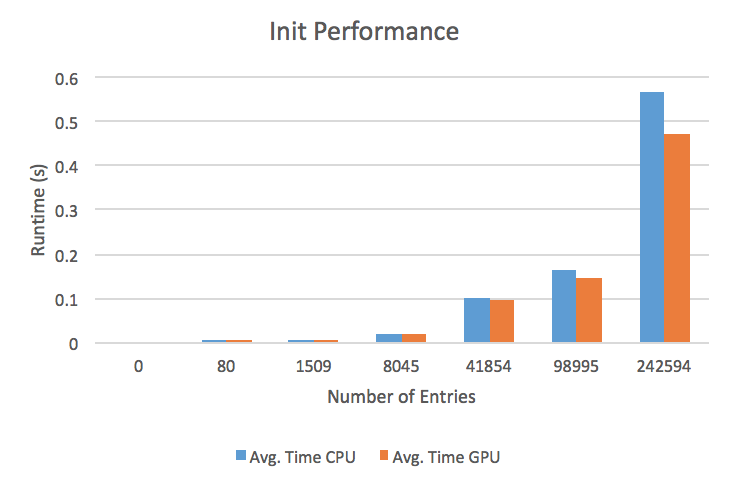
\includegraphics[width=0.7\textwidth]{init_bar.png}
    	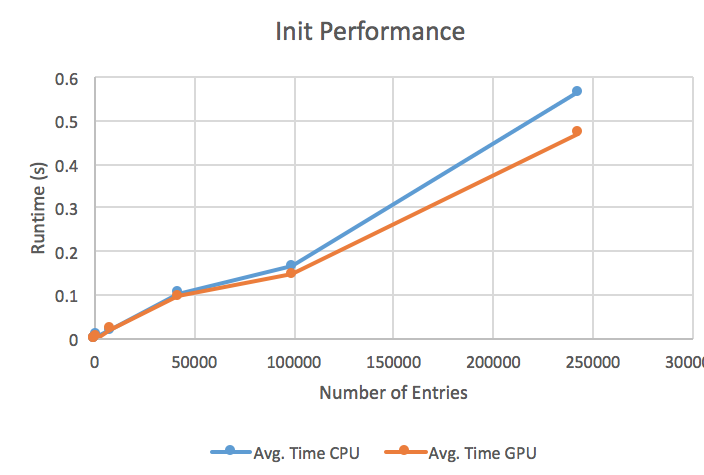
\includegraphics[width=0.7\textwidth]{init_line.png}
    	\end{figure}

\subsection{G4double SampleLin()}% Test Cases Done
	\subsubsection{Test Description}
	 Performs samples of the vector with a linear interpolation scheme.
	
	\subsubsection{Test Inputs}
		\begin{table}[H]
		\centering
		\caption{Unit Tests - \texttt{SampleLin}}\label{SampleLin_unit}
		\begin{tabular}{lll}
		\toprule
		\multirow{2}{*}{\bf Test \#}  & \multicolumn{1}{c}{\bf Inputs}\\
		& \bf \texttt{N/A}\\\midrule
		\refstepcounter{TestCounter}\arabic{TestCounter}\label{SampleLin_0} & N/A \\
		\bottomrule
		\end{tabular}
		\end{table}
	
	\subsubsection{Test Results}
		\begin{table}[H]
		\centering
		\caption{Test Results -- SampleLin}\label{SampleLin_acc}
		\begin{tabular}{clllllll}
		\toprule
		\multirow{2}{*}{\bf Test \#} & \multicolumn{7}{c}{\bf Test Result}\\
		& vec0 & vec1 & vec2 & vec3 & vec4 & vec5 & vec6\\\midrule
		\ref{SampleLin_0} & Pass & Pass & Pass & Pass & Pass & Pass & Pass\\
		\bottomrule
		\end{tabular}
		\end{table}

	\subsubsection{Performance}
		This method is not computationally heavy, so performance data was not included.
		
%\subsection{IntegrateAndNormalise}
%	\subsubsection{Unit Tests}
%		\begin{table}[H]
%		\centering
%		\caption{Unit Tests}\label{IntAndNorm_unit}
%		\begin{tabular}{lll}
%		\toprule
%		\bf Test \# & Code & \bf Description\\\midrule
%		\stepcounter{TestCounter}\arabic{TestCounter}\label{IntAndNorm_0} & Empty.IntegrateAndNormalise() & Integrate and normalize an empty Vector\\
%		\stepcounter{TestCounter}\arabic{TestCounter}\label{IntAndNorm_1} & D.IntegrateAndNormalise() & Integrate normalize a Vector\\
%		\bottomrule
%		\end{tabular}
%		\end{table}
%	\subsubsection{Accuracy}
%		\begin{table}[H]
%		\centering
%		\caption{Accuracy}\label{IntAndNorm_acc}
%		\begin{tabular}{lll}
%		\toprule
%		\bf Test \# & Status \\\midrule
%		\ref{IntAndNorm_0} & Pass\\
%		\ref{IntAndNorm_1} & Pass\\
%		\bottomrule
%		\end{tabular}
%		\end{table}
%	\subsubsection{Performance}
%		This method is not computationally heavy, so performance data was not included.
		
%\subsection{Integrate}
%	\subsubsection{Unit Tests}
%		\begin{table}[H]
%		\centering
%		\caption{Unit Tests}\label{Integrate_unit}
%		\begin{tabular}{lll}
%		\toprule
%		\bf Test \# & Code & \bf Description\\\midrule
%		\refstepcounter{TestCounter}\arabic{TestCounter}\label{Integrate_0} & Empty.Integrate() & Integrate an empty Vector\\
%		\refstepcounter{TestCounter}\arabic{TestCounter}\label{Integrate_1} & D.Integrate() & Integrate a Vector\\
%		\bottomrule
%		\end{tabular}
%		\end{table}
%	\subsubsection{Accuracy}
%		\begin{table}[H]
%		\centering
%		\caption{Accuracy}\label{Integrate_acc}
%		\begin{tabular}{lll}
%		\toprule
%		\bf Test \# & Status \\\midrule
%		\ref{Integrate_0} & Pass\\
%		\ref{Integrate_1} & Pass\\
%		\bottomrule
%		\end{tabular}
%		\end{table}
%	\subsubsection{Performance}
%
%\subsection{IntegrateAndNormalise}
%	\subsubsection{Unit Tests}
%		\begin{table}[H]
%		\centering
%		\caption{Unit Tests}\label{IntAndNorm_unit}
%		\begin{tabular}{lll}
%		\toprule
%		\bf Test \# & Code & \bf Description\\\midrule
%		\stepcounter{TestCounter}\arabic{TestCounter}\label{IntAndNorm_0} & Empty.IntegrateAndNormalise() & Integrate and normalize an empty Vector\\
%		\stepcounter{TestCounter}\arabic{TestCounter}\label{IntAndNorm_1} & D.IntegrateAndNormalise() & Integrate normalize a Vector\\
%		\bottomrule
%		\end{tabular}
%		\end{table}
%	\subsubsection{Accuracy}
%		\begin{table}[H]
%		\centering
%		\caption{Accuracy}\label{IntAndNorm_acc}
%		\begin{tabular}{lll}
%		\toprule
%		\bf Test \# & Status \\\midrule
%		\ref{IntAndNorm_0} & Pass\\
%		\ref{IntAndNorm_1} & Pass\\
%		\bottomrule
%		\end{tabular}
%		\end{table}
%	\subsubsection{Performance}

\subsection{void Times(G4double factor)} % Test Cases done
	\subsubsection{Test Description}
	Multiplies every element in the vector by \texttt{factor}.
	
	\subsubsection{Test Inputs}
		\begin{table}[H]
		\centering
		\caption{Unit Tests - \texttt{Times}}\label{Times_unit}
		\begin{tabular}{lll}
		\toprule
		\multirow{2}{*}{\bf Test \#}  & \multicolumn{1}{c}{\bf Inputs}\\
		& \bf \texttt{factor}\\\midrule
		\refstepcounter{TestCounter}\arabic{TestCounter}\label{Times_0} & r1\\
		\refstepcounter{TestCounter}\arabic{TestCounter}\label{Times_1} & r2\\
		\refstepcounter{TestCounter}\arabic{TestCounter}\label{Times_2} & r3\\
		\refstepcounter{TestCounter}\arabic{TestCounter}\label{Times_3} & r4\\
		\refstepcounter{TestCounter}\arabic{TestCounter}\label{Times_4} & r5\\
		\bottomrule
		\end{tabular}
		\end{table}
	
	\subsubsection{Test Results}
		\begin{table}[H]
		\centering
		\caption{Test Results -- Times}\label{Times_acc}
		\begin{tabular}{clllllll}
		\toprule
		\multirow{2}{*}{\bf Test \#} & \multicolumn{7}{c}{\bf Test Result}\\
		& vec0 & vec1 & vec2 & vec3 & vec4 & vec5 & vec6\\\midrule
		\ref{Times_0} & Pass & Pass & Pass & Pass & Pass & Pass & Pass\\
		\ref{Times_1} & Pass & Pass & Pass & Pass & Pass & Pass & Pass\\
		\ref{Times_2} & Pass & Pass & Pass & Pass & Pass & Pass & Pass\\
		\ref{Times_3} & Pass & Pass & Pass & Pass & Pass & Pass & Pass\\
		\ref{Times_4} & Pass & Pass & Pass & Pass & Pass & Pass & Pass\\
		\bottomrule
		\end{tabular}
		\end{table}

	\subsubsection{Performance}
    	\begin{figure}[H]
    	\centering
    	\caption{Performance results for \texttt{Times} function}\label{figPerformanceTimes}
    	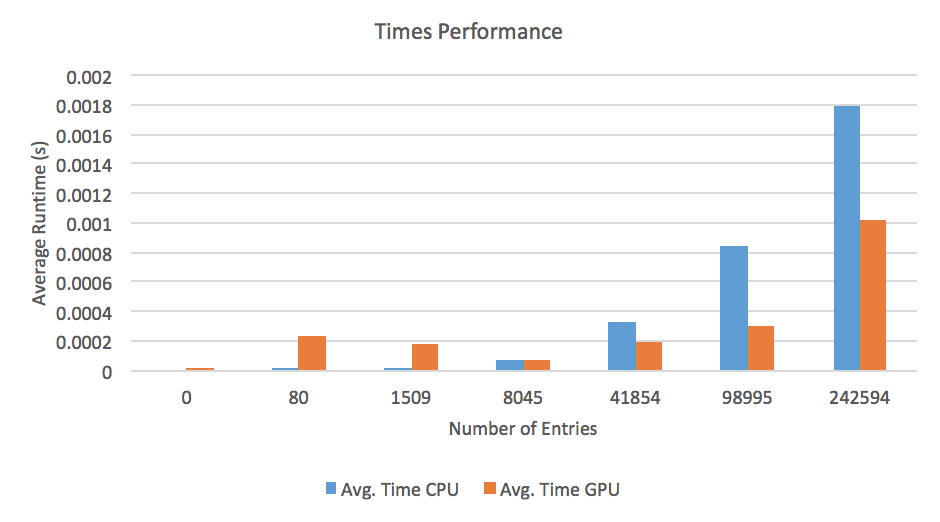
\includegraphics[width=0.7\textwidth]{times_bar.png}
    	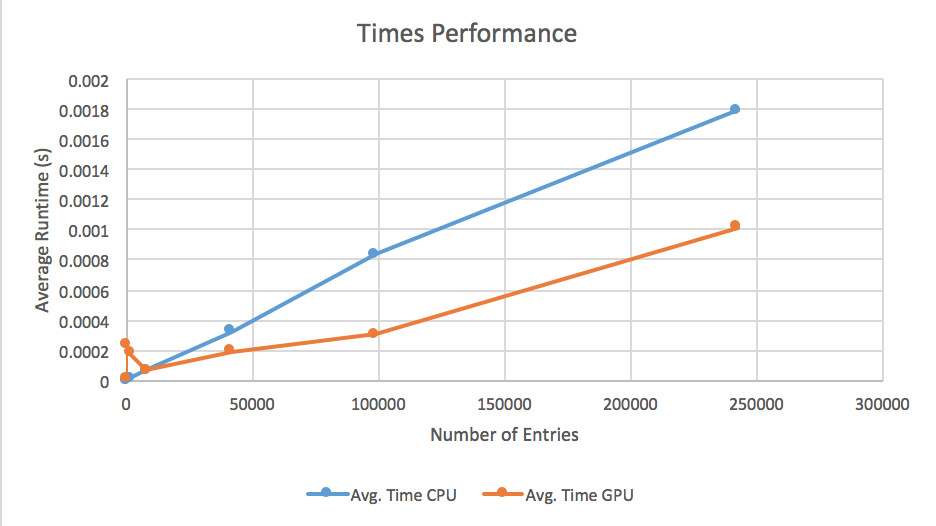
\includegraphics[width=0.7\textwidth]{times_line.png}
    	\end{figure}

%\subsection{GetXsecBuffer}
%	\begin{table}[H]
%	\centering
%	\caption{General Unit Test Variables}\label{buffer_table}
%	\begin{tabular}{lll}
%	\toprule
%		\bf Name & \bf Size & Description\\\midrule 
%		emptyBuff 	& 0		& Array with no queries\\	
%		singleBuff 	& 1		& Array with a single query\\
%		smallbuff	& 50		& Array with a small number of queries\\
%		normalBuff	& 1000	& Array with a moderate number of queries\\
%		largeBuff	& 10000	& Array with a large amount of queries\\
%		negBuff	& 50		& Array of queries with negative values\\
%		zeroBuff	& 50		& Array of queries with values of zero\\
%		highBuff	& 50		& Array of queries with values larger than the highest energy in the vector\\
%	\bottomrule		
%	\end{tabular}
%	\end{table}
%	\subsubsection{Unit Tests}
%		\begin{table}[H]
%		\centering
%		\caption{Unit Tests}\label{xSecBuffer_unit}
%		\begin{tabular}{lll}
%		\toprule
%		\bf Test \# & Code & \bf Description\\\midrule
%		\refstepcounter{TestCounter}\arabic{TestCounter} \label{xSecBuffer_0} & D.GetXsecBuffer(normalBuff, -1) &  buffer with a negative size\\
%		\refstepcounter{TestCounter}\arabic{TestCounter} \label{xSecBuffer_1} & Empty.GetXsecBuffer(emptyBuff, 0) &  Empty buffer of xSec queries to an empty vector\\
%		\refstepcounter{TestCounter}\arabic{TestCounter} \label{xSecBuffer_2} & Empty.GetXsecBuffer(normalBuff, 1000) &  Normal buffer of xSec queries to an empty vector\\
%		\refstepcounter{TestCounter}\arabic{TestCounter} \label{xSecBuffer_3} & D.GetXsecBuffer(emptyBuff, 0) &  Empty buffer of xSec queries\\
%		\refstepcounter{TestCounter}\arabic{TestCounter} \label{xSecBuffer_4} & D.GetXsecBuffer(smalllBuff, 50) &  Small number of queries\\
%		\refstepcounter{TestCounter}\arabic{TestCounter} \label{xSecBuffer_5} & D.GetXsecBuffer(normalBuff, 1000) &  Normal case\\
%		\refstepcounter{TestCounter}\arabic{TestCounter} \label{xSecBuffer_6} & D.GetXsecBuffer(highBuff, 10000) &  Large number of queries\\
%		\refstepcounter{TestCounter}\arabic{TestCounter} \label{xSecBuffer_7} & D.GetXsecBuffer(negBuff, 1000) &  Buffer of negative xSec queries\\
%		\refstepcounter{TestCounter}\arabic{TestCounter} \label{xSecBuffer_8} & D.GetXsecBuffer(emptyBuff, 1000) &  Buffer of zeros\\
%		\refstepcounter{TestCounter}\arabic{TestCounter} \label{xSecBuffer_9} & D.GetXsecBuffer(highBuff, 0) & Buffer of high valued xSec queries\\
%		\bottomrule
%		\end{tabular}
%		\end{table}
%	\subsubsection{Accuracy}
%		\begin{table}[H]
%		\centering
%		\caption{Accuracy}\label{xSecBuffer_acc}
%		\begin{tabular}{lll}
%		\toprule
%		\bf Test \# & Status \\\midrule
%		\ref{xSecBuffer_0} & Pass\\
%		\ref{xSecBuffer_1} & Pass\\
%		\ref{xSecBuffer_2} & Pass\\
%		\ref{xSecBuffer_3} & Pass\\
%		\ref{xSecBuffer_4} & Pass\\
%		\ref{xSecBuffer_5} & Pass\\
%		\ref{xSecBuffer_6} & Pass\\
%		\ref{xSecBuffer_7} & Pass\\
%		\ref{xSecBuffer_8} & Pass\\
%		\ref{xSecBuffer_9} & Pass\\
%		\bottomrule
%		\end{tabular}
%		\end{table}
%	\subsubsection{Performance}
%		This method is not computationally heavy, so performance data was not included.
		
%\subsection{GetXsecBuffer} 
%	\begin{table}[H]
%	\centering
%	\caption{General Unit Test Variables}\label{buffer_table}
%	\begin{tabular}{lll}
%	\toprule
%		\bf Name & \bf Size & Description\\\midrule 
%		emptyBuff 	& 0		& Array with no queries\\	
%		singleBuff 	& 1		& Array with a single query\\
%		smallbuff	& 50		& Array with a small number of queries\\
%		normalBuff	& 1000	& Array with a moderate number of queries\\
%		largeBuff	& 10000	& Array with a large amount of queries\\
%		negBuff	& 50		& Array of queries with negative values\\
%		zeroBuff	& 50		& Array of queries with values of zero\\
%		highBuff	& 50		& Array of queries with values larger than the highest energy in the vector\\
%	\bottomrule		
%	\end{tabular}
%	\end{table}
%	\subsubsection{Unit Tests}
%		\begin{table}[H]
%		\centering
%		\caption{Unit Tests}\label{xSecBuffer_unit}
%		\begin{tabular}{lll}
%		\toprule
%		\bf Test \# & Code & \bf Description\\\midrule
%		\refstepcounter{TestCounter}\arabic{TestCounter} \label{xSecBuffer_0} & D.GetXsecBuffer(normalBuff, -1) &  buffer with a negative size\\
%		\refstepcounter{TestCounter}\arabic{TestCounter} \label{xSecBuffer_1} & Empty.GetXsecBuffer(emptyBuff, 0) &  Empty buffer of xSec queries to an empty vector\\
%		\refstepcounter{TestCounter}\arabic{TestCounter} \label{xSecBuffer_2} & Empty.GetXsecBuffer(normalBuff, 1000) &  Normal buffer of xSec queries to an empty vector\\
%		\refstepcounter{TestCounter}\arabic{TestCounter} \label{xSecBuffer_3} & D.GetXsecBuffer(emptyBuff, 0) &  Empty buffer of xSec queries\\
%		\refstepcounter{TestCounter}\arabic{TestCounter} \label{xSecBuffer_4} & D.GetXsecBuffer(smalllBuff, 50) &  Small number of queries\\
%		\refstepcounter{TestCounter}\arabic{TestCounter} \label{xSecBuffer_5} & D.GetXsecBuffer(normalBuff, 1000) &  Normal case\\
%		\refstepcounter{TestCounter}\arabic{TestCounter} \label{xSecBuffer_6} & D.GetXsecBuffer(highBuff, 10000) &  Large number of queries\\
%		\refstepcounter{TestCounter}\arabic{TestCounter} \label{xSecBuffer_7} & D.GetXsecBuffer(negBuff, 1000) &  Buffer of negative xSec queries\\
%		\refstepcounter{TestCounter}\arabic{TestCounter} \label{xSecBuffer_8} & D.GetXsecBuffer(emptyBuff, 1000) &  Buffer of zeros\\
%		\refstepcounter{TestCounter}\arabic{TestCounter} \label{xSecBuffer_9} & D.GetXsecBuffer(highBuff, 0) & Buffer of high valued xSec queries\\
%		\bottomrule
%		\end{tabular}
%		\end{table}
%	\subsubsection{Accuracy}
%		\begin{table}[H]
%		\centering
%		\caption{Accuracy}\label{xSecBuffer_acc}
%		\begin{tabular}{lll}
%		\toprule
%		\bf Test \# & Status \\\midrule
%		\ref{xSecBuffer_0} & Pass\\
%		\ref{xSecBuffer_1} & Pass\\
%		\ref{xSecBuffer_2} & Pass\\
%		\ref{xSecBuffer_3} & Pass\\
%		\ref{xSecBuffer_4} & Pass\\
%		\ref{xSecBuffer_5} & Pass\\
%		\ref{xSecBuffer_6} & Pass\\
%		\ref{xSecBuffer_7} & Pass\\
%		\ref{xSecBuffer_8} & Pass\\
%		\ref{xSecBuffer_9} & Pass\\
%		\bottomrule
%		\end{tabular}
%		\end{table}
%	\subsubsection{Performance}

\subsection{void ThinOut(G4double precision)} % Test Cases done 
	\subsubsection{Test Description}
	Removes any element from the vector whose neighbor is closer than \texttt{precision}.
	
	\subsubsection{Test Inputs}
		\begin{table}[H]
		\centering
		\caption{Unit Tests - \texttt{ThinOut}}\label{ThinOut_unit}
		\begin{tabular}{lll}
		\toprule
		\multirow{2}{*}{\bf Test \#}  & \multicolumn{1}{c}{\bf Inputs}\\
		& \bf \texttt{factor}\\\midrule
		\refstepcounter{TestCounter}\arabic{TestCounter}\label{ThinOut_0} & r1\\
		\refstepcounter{TestCounter}\arabic{TestCounter}\label{ThinOut_1} & r2\\
		\refstepcounter{TestCounter}\arabic{TestCounter}\label{ThinOut_2} & r3\\
		\refstepcounter{TestCounter}\arabic{TestCounter}\label{ThinOut_3} & r4\\
		\refstepcounter{TestCounter}\arabic{TestCounter}\label{ThinOut_4} & r5\\
		\bottomrule
		\end{tabular}
		\end{table}
	
	\subsubsection{Test Results}
		\begin{table}[H]
		\centering
		\caption{Test Results -- ThinOut}\label{ThinOut_acc}
		\begin{tabular}{clllllll}
		\toprule
		\multirow{2}{*}{\bf Test \#} & \multicolumn{7}{c}{\bf Test Result}\\
		& vec0 & vec1 & vec2 & vec3 & vec4 & vec5 & vec6\\\midrule
		\ref{ThinOut_0} & Pass & Pass & Pass & Pass & Pass & Pass & Pass\\
		\ref{ThinOut_1} & Pass & Pass & Pass & Pass & Pass & Pass & Pass\\
		\ref{ThinOut_2} & Pass & Pass & Pass & Pass & Pass & Pass & Pass\\
		\ref{ThinOut_3} & Pass & Pass & Pass & Pass & Pass & Pass & Pass\\
		\ref{ThinOut_4} & Pass & Pass & Pass & Pass & Pass & Pass & Pass\\
		\bottomrule
		\end{tabular}
		\end{table}

	\subsubsection{Performance}
		This method is not computationally heavy, so performance data was not included.

\subsection{G4double Sample()}% Test Cases Done
	\subsubsection{Test Description}
	  Performs samples of the vector according to interpolation its interpolation scheme.
	
	\subsubsection{Test Inputs}
		\begin{table}[H]
		\centering
		\caption{Unit Tests - \texttt{Sample}}\label{Sample_unit}
		\begin{tabular}{lll}
		\toprule
		\multirow{2}{*}{\bf Test \#}  & \multicolumn{1}{c}{\bf Inputs}\\
		& \bf \texttt{N/A}\\\midrule
		\refstepcounter{TestCounter}\arabic{TestCounter}\label{Sample_0} & N/A \\
		\bottomrule
		\end{tabular}
		\end{table}
	
	\subsubsection{Test Results}
		\begin{table}[H]
		\centering
		\caption{Test Results -- Sample}\label{Sample_acc}
		\begin{tabular}{clllllll}
		\toprule
		\multirow{2}{*}{\bf Test \#} & \multicolumn{7}{c}{\bf Test Result}\\
		& vec0 & vec1 & vec2 & vec3 & vec4 & vec5 & vec6\\\midrule
		\ref{Sample_0} & Pass & Pass & Pass & Pass & Pass & Pass & Pass\\
		\bottomrule
		\end{tabular}
		\end{table}

	\subsubsection{Performance}
		This method is not computationally heavy, so performance data was not included.
		
%\subsection{GetIntegral}
%	\subsubsection{Unit Tests}
%		\begin{table}[H]
%		\centering
%		\caption{Unit Tests}\label{_unit}
%		\begin{tabular}{lll}
%		\toprule
%		\bf Test \# & Code & \bf Description\\\midrule
%		\refstepcounter{TestCounter}\arabic{TestCounter} & Code goes here & Description goes here\\
%		\bottomrule
%		\end{tabular}
%		\end{table}
%	\subsubsection{Accuracy}
%		\begin{table}[H]
%		\centering
%		\caption{Accuracy}\label{_acc}
%		\begin{tabular}{lll}
%		\toprule
%		\bf Test \# & CPU & GPU \\\midrule
%		\arabic{TestCounter} & CPU time & GPU time\\
%		\bottomrule
%		\end{tabular}
%		\end{table}
%	\subsubsection{Performance}

\subsection{SetPoint} 
	\subsubsection{Unit Tests}
		\begin{itemize}
			\item ``rPoint" is a random G4ParticleHPDataPoint
			\item ``nPoint" is a negative G4ParticleHPDataPoint
			\item ``zPoint" is a zero G4ParticleHPDataPoint
		\end{itemize}
		\begin{table}[H]
		\centering
		\caption{Unit Tests}\label{SetPoint_unit}
		\begin{tabular}{lll}
		\toprule
		\bf Test \# & Code & \bf Description\\\midrule
		\refstepcounter{TestCounter}\arabic{TestCounter}\label{SetPoint_0} & Empty.SetPoint(-1, rPoint) & Set a point at a negative index of an empty vector\\
		\refstepcounter{TestCounter}\arabic{TestCounter}\label{SetPoint_1} & Empty.SetPoint(0, rPoint) & Set a point at a the first index of an empty vector\\
		\refstepcounter{TestCounter}\arabic{TestCounter}\label{SetPoint_2} & Empty.SetPoint(1, rPoint) & Set a point at an index out of bounds of an empty vector\\
		\refstepcounter{TestCounter}\arabic{TestCounter}\label{SetPoint_3} & D.SetPoint(-1, rPoint) & Set a point at a negative index\\
		\refstepcounter{TestCounter}\arabic{TestCounter}\label{SetPoint_4} & D.SetPoint(0, rPoint) & Set a point at a the first index\\
		\refstepcounter{TestCounter}\arabic{TestCounter}\label{SetPoint_5} & D.SetPoint(n/2, rPoint) & Set a point at an index within the vector\\
		\refstepcounter{TestCounter}\arabic{TestCounter}\label{SetPoint_6} & D.SetPoint(n-1, rPoint) & Set a point at the last index\\
		\refstepcounter{TestCounter}\arabic{TestCounter}\label{SetPoint_7} & D.SetPoint(n, rPoint) & Set a point at an index our of bounds\\
		\refstepcounter{TestCounter}\arabic{TestCounter}\label{SetPoint_8} & D.SetPoint(0, nPoint) & Set a negative point\\
		\refstepcounter{TestCounter}\arabic{TestCounter}\label{SetPoint_9} & D.SetPoint(0, zPoint) & Set a zero point\\
		\bottomrule
		\end{tabular}
		\end{table}
	\subsubsection{Accuracy}
		\begin{table}[H]
		\centering
		\caption{Accuracy}\label{SetPoint_acc}
		\begin{tabular}{lll}
		\toprule
		\bf Test \# & Status \\\midrule
		\ref{SetPoint_0} & Pass\\
		\ref{SetPoint_1} & Pass\\
		\ref{SetPoint_2} & Pass\\
		\ref{SetPoint_3} & Pass\\
		\ref{SetPoint_4} & Pass\\
		\ref{SetPoint_5} & Pass\\
		\ref{SetPoint_6} & Pass\\
		\ref{SetPoint_7} & Pass\\
		\ref{SetPoint_8} & Pass\\
		\ref{SetPoint_9} & Pass\\
		\bottomrule
		\end{tabular}
		\end{table}
	\subsubsection{Performance}
		This method is not computationally heavy, so performance data was not included.

%\subsection{Merge}
%	\subsubsection{Unit Tests}
%		\begin{table}[!htbp]
%		\centering
%		\caption{Unit Tests}\label{Merge_unit}
%		\begin{tabular}{lll}
%		\toprule
%		\bf Test \# & Code & \bf Description\\\midrule
%		\refstepcounter{TestCounter}\arabic{TestCounter} & Code goes here & Description goes here\\
%		\bottomrule
%		\end{tabular}
%		\end{table}
%	\subsubsection{Accuracy}
%		\begin{table}[!htbp]
%		\centering
%		\caption{Accuracy}\label{Merge_acc}
%		\begin{tabular}{lll}
%		\toprule
%		\bf Test \# & Status \\\midrule
%		\arabic{TestCounter} & Pass\\
%		\bottomrule
%		\end{tabular}
%		\end{table}
%	\subsubsection{Performance}

\subsection{G4double Get15percentBorder()} % Test Cases Done
	\subsubsection{Test Description}
	 Returns the integral from each data point to the last data point and returns the first one within 
15\% of the last data point.
	
	\subsubsection{Test Inputs}
		\begin{table}[H]
		\centering
		\caption{Unit Tests - \texttt{Get15percentBorder}}\label{Get15percentBorder_unit}
		\begin{tabular}{lll}
		\toprule
		\multirow{2}{*}{\bf Test \#}  & \multicolumn{1}{c}{\bf Inputs}\\
		& \bf \texttt{N/A}\\\midrule
		\refstepcounter{TestCounter}\arabic{TestCounter}\label{Get15percentBorder_0} & N/A \\
		\bottomrule
		\end{tabular}
		\end{table}
	
	\subsubsection{Test Results}
		\begin{table}[H]
		\centering
		\caption{Test Results -- Get15percentBorder}\label{Get15percentBorder_acc}
		\begin{tabular}{clllllll}
		\toprule
		\multirow{2}{*}{\bf Test \#} & \multicolumn{7}{c}{\bf Test Result}\\
		& vec0 & vec1 & vec2 & vec3 & vec4 & vec5 & vec6\\\midrule
		\ref{Get15percentBorder_0} & Pass & Pass & Pass & Pass & Pass & Pass & Pass\\
		\bottomrule
		\end{tabular}
		\end{table}

	\subsubsection{Performance}
		This method is not computationally heavy, so performance data was not included.
		
\subsection{G4double Get50percentBorder()}% Test Cases Done
	\subsubsection{Test Description}
	 Returns the integral from each data point to the last data point and returns the first one within 
50\% of the last data point.
	
	\subsubsection{Test Inputs}
		\begin{table}[H]
		\centering
		\caption{Unit Tests - \texttt{Get50percentBorder}}\label{Get50percentBorder_unit}
		\begin{tabular}{lll}
		\toprule
		\multirow{2}{*}{\bf Test \#}  & \multicolumn{1}{c}{\bf Inputs}\\
		& \bf \texttt{N/A}\\\midrule
		\refstepcounter{TestCounter}\arabic{TestCounter}\label{Get50percentBorder_0} & N/A \\
		\bottomrule
		\end{tabular}
		\end{table}
	
	\subsubsection{Test Results}
		\begin{table}[H]
		\centering
		\caption{Test Results -- Get50percentBorder}\label{Get50percentBorder_acc}
		\begin{tabular}{clllllll}
		\toprule
		\multirow{2}{*}{\bf Test \#} & \multicolumn{7}{c}{\bf Test Result}\\
		& vec0 & vec1 & vec2 & vec3 & vec4 & vec5 & vec6\\\midrule
		\ref{Get50percentBorder_0} & Pass & Pass & Pass & Pass & Pass & Pass & Pass\\
		\bottomrule
		\end{tabular}
		\end{table}

	\subsubsection{Performance}
		This method is not computationally heavy, so performance data was not included.
		
% =============================== Section =============================== %
\section{System Tests}
\subsection{Summary of Tests Performed}
System tests will be performed by running the sample code packaged with the GEANT4 installation. The Hadr04 example will be run with different materials (i.e water, uranium) and number of events. The values and conditions that are changed per test are detailed in the table below.\\ \\

\begin{center}
\begin{longtable}{cc >{\raggedright\arraybackslash}p{2.8cm}>{\raggedright\arraybackslash}p{3cm}>{\raggedright\arraybackslash}p{4.5cm}}
\caption{System Tests}\label{Table_SystemTests}\\
\toprule

\bf Test \# & \bf Initial State & \bf Inputs & \bf Outputs & \bf Description\\\midrule
\refstepcounter{TestCounter}\arabic{TestCounter}\label{sys1}
& Fresh start up
& Events = 2000
Material = Water
& Same output as non-GPU GEANT4 
&  HADR04 no changes\\\midrule

\refstepcounter{TestCounter}\arabic{TestCounter}\label{sys2}
& Fresh start up 
& Events = 2000
Material = Uranium
& Same output as non-GPU GEANT4 
& HADR04 -- basic example\\\midrule

\refstepcounter{TestCounter}\arabic{TestCounter}\label{sys3}
& Fresh start up 
& Events = 600
Material = Water
& Same output as non-GPU GEANT4 
& HADR04 -- Shorter test \\\midrule

\refstepcounter{TestCounter}\arabic{TestCounter}\label{sys4}
& Fresh start up 
& Events = 600
Material = Uranium
& Same output as non-GPU GEANT4 
& HADR04 -- Shorter test \\\midrule

\refstepcounter{TestCounter}\arabic{TestCounter}\label{sys5}
& Fresh start up 
& Events = 20000
Material = Uranium
& Same output as non-GPU GEANT4 
& HADR04 -- Long simulation stress Test\\\midrule

\refstepcounter{TestCounter}\arabic{TestCounter}\label{sys6}
& Fresh start up 
& Events = 0
Material = Uranium
& Same output as non-GPU GEANT4 
& HADR04 -- no runs,  Edge case\\

\bottomrule
\end{longtable}
\end{center}
\subsection{System Tests Results}
This section will summarize all of the results from running tests 39 through 44. Each test has an accuracy section as well as a performance section. The accuracy of the results will be based on how well the values generated on the GPU match up with the values generated on the CPU. The performance metrics used will include user, system and real time required to run each  system test.

\subsection{System test \# \ref{sys1}}
This test simply runs the Hadr04 example on both the GPU and the CPU without changing the source files. The code for this example is bundled with the GEANT4 installation.\\
	\subsubsection{Accuracy}
		\begin{table}[!htbp]
		\centering
		\caption{Accuracy Test \# \ref{sys1}}\label{_acc}
		\begin{tabular}{llll}
		\toprule
		\bf Data & CPU Values & GPU Values & Difference\\\midrule
		\bf Process Calls&&&\\
		hadElastic&423181&441475&NA\\
		nCapture&1998&2000&NA\\
		neutronInelastic&2&0&NA\\ 
		\bf Parcours of incident neutron&&&\\
		collisions&212.59&221.74&NA\\
		track length&93.387 cm&96.948 cm&NA\\
		time of flight&202.14 mus&210.93 mus&NA\\
		\bf Generated particles&&&\\
		\underline{C14}&&&\\
		\# of particles&2&NA&NA\\
		Emean&404.13 keV&NA&NA\\
		Range&404.02 keV-404.25 keV&NA&NA\\
		\underline{O16}&&&\\
		\# of particles&5948&6146&NA\\
		Emean&39.577 keV&40.32 keV&NA\\
		Range&0.73669 meV-447.06 keV&1.417 meV-446.59 keV&NA\\
		\underline{O17}&&&\\
		\# of particles&4&NA&NA\\
		Emean&1.4823 keV&NA&NA\\
		Range&187.15 eV-4.9785 keV&NA&NA\\
		\underline{O18}&&&\\
		\# of particles&3&NA&NA\\
		Emean&52.362&NA&NA\\
		Range&9.3256 eV-153.04 keV&NA&NA\\
		\underline{Alpha}&&&\\
		\# of particles&2&NA&NA\\
		Emean&1.4146 MeV&NA&NA\\
		Range&1.4145 MeV-1.4147 MeV&NA&NA\\
		\underline{Deuteron}&&&\\
		\# of particles&1996&NA&NA\\
		Emean&1.3185 keV&NA&NA\\
		Range&237.52 meV-1.7025 keV&NA&NA\\
		\underline{Gamma}&&&\\
		\# of particles&2000&NA&NA\\
		Emean&2.2239 MeV&NA&NA\\
		Range&870.8 keV-4.1431 MeV&NA&NA\\
		\underline{Proton}&&&\\
		\# of particles&45355&NA&NA\\
		Emean&83.046 keV&NA&NA\\
		Range&0.13176 meV-1.9993 MeV&NA&NA\\
		\end{tabular}
		\end{table}
		\break
	\subsubsection{Performance}
		\begin{table}[!htbp]
		\centering
		\caption{Performance Test \# \ref{sys1}}\label{_acc}
		\begin{tabular}{lll}
		\toprule
		Type&CPU Time& GPU Time\\\midrule
		User&55.09s&NA\\
		Real&55.19s&NA\\
		System&0.05s&NA\\
		\end{tabular}
		\end{table}
\break
\subsection{System test \#  \ref{sys2}}
This test simply runs the Hadr04 example on both the GPU and the CPU without changing the source files. The code for this example is bundled with the GEANT4 installation.\\
	\subsubsection{Accuracy}
		\begin{table}[!htbp]
		\centering
		\caption{Accuracy Test \# \ref{sys2}}\label{_acc}
		\begin{tabular}{llll}
		\toprule
		\bf Data & CPU Values & GPU Values & Difference\\\midrule
		\bf Process Calls&&&\\
		hadElastic&NA&NA&NA\\
		nCapture&NA&NA&NA\\
		neutronInelastic&NA&NA&NA\\ 
		\bf Parcours of incident neutron&&&\\
		collisions&NA&NA&NA\\
		track length&NA&NA&NA\\
		time of flight&NA&NA&NA\\
		\bf Generated particles&&&\\
		\underline{U23}5&&&\\
		\# of particles&NA&NA&NA\\
		Emean&NA&NA&NA\\
		Range&NA&NA&NA\\
		\underline{U238}&&&\\
		\# of particles&NA&NA&NA\\
		Emean&NA&NA&NA\\
		Range&NA&NA&NA\\
		\underline{U239}&&&\\
		\# of particles&NA&NA&NA\\
		Emean&NA&NA&NA\\
		Range&NA&NA&NA\\
		\underline{Gamma}&&&\\
		\# of particles&NA&NA&NA\\
		Emean&NA&NA&NA\\
		Range&NA&NA&NA\\
		\underline{Neutron}&&&\\
		\# of particles&NA&NA&NA\\
		Emean&NA&NA&NA\\
		Range&NA&NA&NA\\
		\end{tabular}
		\end{table}
		\break
	\subsubsection{Performance}
		\begin{table}[!htbp]
		\centering
		\caption{Performance Test \# \ref{sys2}}\label{_acc}
		\begin{tabular}{lll}
		\toprule
		Type&CPU Time& GPU Time\\\midrule
		User&NA&NA\\
		Real&NA&NA\\
		System&NA&NA\\
		\end{tabular}
		\end{table}
\subsection{System test \#  \ref{sys3}}
This test simply runs the Hadr04 example on both the GPU and the CPU without changing the source files. The code for this example is bundled with the GEANT4 installation.\\
\break
	\subsubsection{Accuracy}
		\begin{table}[!htbp]
		\centering
		\caption{Accuracy Test \# \ref{sys3}}\label{_acc}
		\begin{tabular}{llll}
		\toprule
		\bf Data & CPU Values & GPU Values & Difference\\\midrule
		\bf Process Calls&&&\\
		hadElastic&NA&NA&NA\\
		nCapture&NA&NA&NA\\
		neutronInelastic&NA&NA&NA\\ 
		\bf Parcours of incident neutron&&&\\
		collisions&NA&NA&NA\\
		track length&NA&NA&NA\\
		time of flight&NA&NA&NA\\
		\bf Generated particles&&&\\
		\underline{O16}&&&\\
		\# of particles&NA&NA&NA\\
		Emean&NA&NA&NA\\
		Range&NA&NA&NA\\
		\underline{O17}&&&\\
		\# of particles&NA&NA&NA\\
		Emean&NA&NA&NA\\
		Range&NA&NA&NA\\
		\underline{O18}&&&\\
		\# of particles&NA&NA&NA\\
		Emean&NA&NA&NA\\
		Range&NA&NA&NA\\
		\underline{Deuteron}&&&\\
		\# of particles&NA&NA&NA\\
		Emean&NA&NA&NA\\
		Range&NA&NA&NA\\
		\underline{Gamma}&&&\\
		\# of particles&NA&NA&NA\\
		Emean&NA&NA&NA\\
		Range&NA&NA&NA\\
		\underline{Proton}&&&\\
		\# of particles&NA&NA&NA\\
		Emean&NA&NA&NA\\
		Range&NA&NA&NA\\
		\end{tabular}
		\end{table}
		\break
	\subsubsection{Performance}
		\begin{table}[!htbp]
		\centering
		\caption{Performance Test \# \ref{sys3}}\label{_acc}
		\begin{tabular}{lll}
		\toprule
		Type&CPU Time& GPU Time\\\midrule
		User&NA&NA\\
		Real&NA&NA\\
		System&NA&NA\\
		\end{tabular}
		\end{table}
		
\subsection{System test \#  \ref{sys4}}
This test simply runs the Hadr04 example on both the GPU and the CPU without changing the source files. The code for this example is bundled with the GEANT4 installation.\\
\break
	\subsubsection{Accuracy}
		\begin{table}[!htbp]
		\centering
		\caption{Accuracy Test \# \ref{sys4}}\label{_acc}
		\begin{tabular}{llll}
		\toprule
		\bf Data & CPU Values & GPU Values & Difference\\\midrule
		\bf Process Calls&&&\\
		hadElastic&NA&NA&NA\\
		nCapture&NA&NA&NA\\
		neutronInelastic&NA&NA&NA\\ 
		\bf Parcours of incident neutron&&&\\
		collisions&NA&NA&NA\\
		track length&NA&NA&NA\\
		time of flight&NA&NA&NA\\
		\bf Generated particles&&&\\
		\underline{O16}&&&\\
		\# of particles&NA&NA&NA\\
		Emean&NA&NA&NA\\
		Range&NA&NA&NA\\
		\underline{O17}&&&\\
		\# of particles&NA&NA&NA\\
		Emean&NA&NA&NA\\
		Range&NA&NA&NA\\
		\underline{O18}&&&\\
		\# of particles&NA&NA&NA\\
		Emean&NA&NA&NA\\
		Range&NA&NA&NA\\
		\underline{Deuteron}&&&\\
		\# of particles&NA&NA&NA\\
		Emean&NA&NA&NA\\
		Range&NA&NA&NA\\
		\underline{Gamma}&&&\\
		\# of particles&NA&NA&NA\\
		Emean&NA&NA&NA\\
		Range&NA&NA&NA\\
		\underline{Proton}&&&\\
		\# of particles&NA&NA&NA\\
		Emean&NA&NA&NA\\
		Range&NA&NA&NA\\
		\end{tabular}
		\end{table}
		\break
	\subsubsection{Performance}
		\begin{table}[!htbp]
		\centering
		\caption{Performance Test \# \ref{sys4}}\label{_acc}
		\begin{tabular}{lll}
		\toprule
		Type&CPU Time& GPU Time\\\midrule
		User&NA&NA\\
		Real&NA&NA\\
		System&NA&NA\\
		\end{tabular}
		\end{table}
		
\subsection{System test \#  \ref{sys5}}
This test simply runs the Hadr04 example on both the GPU and the CPU without changing the source files. The code for this example is bundled with the GEANT4 installation.\\
\break
	\subsubsection{Accuracy}
		\begin{table}[!htbp]
		\centering
		\caption{Accuracy Test \# \ref{sys5}}\label{_acc}
		\begin{tabular}{llll}
		\toprule
		\bf Data & CPU Values & GPU Values & Difference\\\midrule
		\bf Process Calls&&&\\
		hadElastic&NA&NA&NA\\
		nCapture&NA&NA&NA\\
		neutronInelastic&NA&NA&NA\\ 
		\bf Parcours of incident neutron&&&\\
		collisions&NA&NA&NA\\
		track length&NA&NA&NA\\
		time of flight&NA&NA&NA\\
		\bf Generated particles&&&\\
		\underline{O16}&&&\\
		\# of particles&NA&NA&NA\\
		Emean&NA&NA&NA\\
		Range&NA&NA&NA\\
		\underline{O17}&&&\\
		\# of particles&NA&NA&NA\\
		Emean&NA&NA&NA\\
		Range&NA&NA&NA\\
		\underline{O18}&&&\\
		\# of particles&NA&NA&NA\\
		Emean&NA&NA&NA\\
		Range&NA&NA&NA\\
		\underline{Deuteron}&&&\\
		\# of particles&NA&NA&NA\\
		Emean&NA&NA&NA\\
		Range&NA&NA&NA\\
		\underline{Gamma}&&&\\
		\# of particles&NA&NA&NA\\
		Emean&NA&NA&NA\\
		Range&NA&NA&NA\\
		\underline{Proton}&&&\\
		\# of particles&NA&NA&NA\\
		Emean&NA&NA&NA\\
		Range&NA&NA&NA\\
		\end{tabular}
		\end{table}
		\break
	\subsubsection{Performance}
		\begin{table}[!htbp]
		\centering
		\caption{Performance Test \# \ref{sys5}}\label{_acc}
		\begin{tabular}{lll}
		\toprule
		Type&CPU Time& GPU Time\\\midrule
		User&NA&NA\\
		Real&NA&NA\\
		System&NA&NA\\
		\end{tabular}
		\end{table}
		
\subsection{System test \#  \ref{sys6}}
This test simply runs the Hadr04 example on both the GPU and the CPU without changing the source files. The code for this example is bundled with the GEANT4 installation.\\
\break
	\subsubsection{Accuracy}
		\begin{table}[!htbp]
		\centering
		\caption{Accuracy Test \# \ref{sys6}}\label{_acc}
		\begin{tabular}{llll}
		\toprule
		\bf Data & CPU Values & GPU Values & Difference\\\midrule
		\bf Process Calls&&&\\
		hadElastic&NA&NA&NA\\
		nCapture&NA&NA&NA\\
		neutronInelastic&NA&NA&NA\\ 
		\bf Parcours of incident neutron&&&\\
		collisions&NA&NA&NA\\
		track length&NA&NA&NA\\
		time of flight&NA&NA&NA\\
		\bf Generated particles&&&\\
		\underline{O16}&&&\\
		\# of particles&NA&NA&NA\\
		Emean&NA&NA&NA\\
		Range&NA&NA&NA\\
		\underline{O17}&&&\\
		\# of particles&NA&NA&NA\\
		Emean&NA&NA&NA\\
		Range&NA&NA&NA\\
		\underline{O18}&&&\\
		\# of particles&NA&NA&NA\\
		Emean&NA&NA&NA\\
		Range&NA&NA&NA\\
		\underline{Deuteron}&&&\\
		\# of particles&NA&NA&NA\\
		Emean&NA&NA&NA\\
		Range&NA&NA&NA\\
		\underline{Gamma}&&&\\
		\# of particles&NA&NA&NA\\
		Emean&NA&NA&NA\\
		Range&NA&NA&NA\\
		\underline{Proton}&&&\\
		\# of particles&NA&NA&NA\\
		Emean&NA&NA&NA\\
		Range&NA&NA&NA\\
		\end{tabular}
		\end{table}
		\break
	\subsubsection{Performance}
		\begin{table}[!htbp]
		\centering
		\caption{Performance Test \# \ref{sys6}}\label{_acc}
		\begin{tabular}{lll}
		\toprule
		Type&CPU Time& GPU Time\\\midrule
		User&NA&NA\\
		Real&NA&NA\\
		System&NA&NA\\
		\end{tabular}
		\end{table}
% =============================== Section =============================== %
\section{Traceability}
The following section is used to highlight the relations of implemented test cases to requirements and modules. In doing so, we hope to draw clear reasoning upon the inclusion of such tests. 
\subsection{Requirements}
Below is a traceability table outlining test cases and the requirements they are related to:\\

\begin{center}
\begin{longtable}{>{\raggedright\arraybackslash}p{0.1\textwidth}>{\raggedright\arraybackslash}p{0.3\textwidth}>{\raggedright\arraybackslash}p{0.5\textwidth}}
\caption{Tests and Requirements Relationship}\label{Table_TestsAndRequirements}
\\\toprule
\bf Test \#  & \bf Description & \bf Requirement\\\toprule
1 & Performance test of functions & Req. \# 4 (Speed and Latency)\\\hline
2 & InitializeVector & Req \# 5 \& 6 \& 7 (Precision \& Reliability \& Robustness)\\\hline
3 & SettersandGetters & Req \# 5 \& 6 \& 7 (Precision \& Reliability \& Robustness)\\\hline
4 & GetXSec & Req \# 5 \& 6 \& 7 (Precision \& Reliability \& Robustness)\\\hline
5 & ThinOut & Req \# 5 \& 6 \& 7 (Precision \& Reliability \& Robustness)\\\hline
6 & Merge & Req \# 5 \& 6 \& 7 (Precision \& Reliability \& Robustness)\\\hline
7 & Sample & Req \# 5 \& 6 \& 7 (Precision \& Reliability \& Robustness)\\\hline
8 & GetBorder & Req \# 5 \& 6 \& 7 (Precision \& Reliability \& Robustness)\\\hline
9 & Integral & Req \# 5 \& 6 \& 7 (Precision \& Reliability \& Robustness)\\\hline
10 & Times & Req \# 5 \& 6\& 7 (Precision \& Reliability \& Robustness)\\\hline
11 & Assignment & Req \# 5 \& 6 \& 7 (Precision \& Reliability \& Robustness)\\\hline
12 & System Test &  Req \# 1 \& 2 \& 8 \& 11 (Adjacent Systems \& Access)\\
\bottomrule
\end{longtable}
\end{center}
\subsection{Modules}
Similarly, the following is a traceability table explicitly relating test cases to modules:\\

\begin{center}
\begin{longtable}{>{\raggedright\arraybackslash}p{0.1\textwidth}>{\raggedright\arraybackslash}p{0.3\textwidth}>{\raggedright\arraybackslash}p{0.5\textwidth}}
\caption{Tests and Modules Relationship}\label{Table_TestsAndModules}
\\\toprule
\bf Test \#  & \bf Description & \bf Module\\\toprule
1 & Performance test of functions & G4ParticleVector\\\hline
2 & InitializeVector & G4ParticleVector\\\hline
3 & SettersandGetters & G4ParticleVector\\\hline
4 & GetXSec & G4ParticleVector\\\hline
5 & ThinOut & G4ParticleVector\\\hline
6 & Merge & G4ParticleVector\\\hline
7 & Sample & G4ParticleVector\\\hline
8 & GetBorder & G4ParticleVector\\\hline
9 & Integral & G4ParticleVector\\\hline
10 & Times & G4ParticleVector\\\hline
11 & Assignment & G4ParticleVector\\\hline
12 & System Test & G4NeutronHPDataPoint \& G4ParticleVector \& CMake Files\\
\bottomrule
\end{longtable}
\end{center}

% =============================== Section =============================== 
% --------------------------- Stuart
\section{Changes after Testing}
Developing the unit testing system illuminated a variety of bugs and changes that needed to be made. These were predominantly related to edge cases -- trying to access indices in arrays that are negative or greater than the number of elements was a common theme. In some of these cases the same case was not covered by Geant4 itself, so the change was made there as well.

\end{document}
